\documentclass{article}
\usepackage{verbatim}
\usepackage{amssymb}
\usepackage{fullpage}
\usepackage{float}
\usepackage{algorithmicx, algorithm}
\usepackage{graphicx}

\graphicspath{{figs/}}
\author{Lucas Roberts}
\date{\today}
\begin{document}
\title{
Why nematologists should use zero-inflated models when modeling count data.  
}

\maketitle

\section{Introduction}


\begin{itemize}
\item Models encompass traditional count data models as special cases and account for excess zeros common in nematology. 
\item Readily available-and often free-software has ready made codes to fit zero-inflated models. 
\item Using Poisson based models when zero-inflation is present leads to biased estimates and larger mean squared errors.   
\end{itemize}

\section{Estimation challenges}

The Bias of an estimator is defined as the expected value of the estimator minus the parameter to be estimated. In the case of count data often the researcher wants to know the rate parameter which indicates an average number of nematodes per unit of soil volume. Let the rate parameter be denoted $\lambda$ and the zero inflation probability be denoted $\phi$. Then if the researchers use the common average of the count data, denoted $\bar{y}$ then the expected value of this estimator is 

\begin{equation}
\mathbb{E}(\bar{y}) = (1-\phi)\lambda.
\end{equation}
Thus the bias of the estimate is 

\begin{equation}
\mathbb{E}(\bar{y}) - \lambda = -\phi\lambda,
\end{equation}
so that the larger the zero-inflation or the rate parameter, the larger the bias of the estimate. Other common approaches are to add 1 to each observed count. If the counts are indeed Poisson distributed, the resultant random variable is a size-biased Poisson. Regardless of the underlying distribution the rate estimate will now be biased by 1. to remove this bias you may safely subtract unity from the final estimate. This does not solve the problem of excess zeroes. Finally, some authors prefer to use a transformed version of the count with a 1 added, some examples are $log(y+1)$ or $\sqrt{2(y+1)}$. Both lead to biased estimators of the underlying rate. The second transform which uses a squared root, has roots in the variance stabilization literature and would be reasonable without the addition of a 1 only if the underlying counts are Poisson distributed.  

One common measure of the closeness of estimators in statistics is the mean squared error (MSE). The MSE is defined as the expected value of the square of the difference between the estimator and the true value of the parameter. Formally, write 
\begin{equation}
MSE(\bar{y}, \lambda) = \mathbb{E}(\bar{y}-\lambda)^2,
\end{equation}
For the average as an estimator of the rate the MSE is 
\begin{equation}
MSE(\bar{y}, \lambda) = \phi^2\lambda^2 + \frac{ \lambda(1-\phi) +\lambda^2(1-\phi)\phi}{n}.
\end{equation}
This last equation tells us that even with an infinite number of samples unless the zero-inflation is non-existent, there will be a bias and the traditional methods will be suboptimal to use in place of estimators of zero-inflated data generating processes. The preceding portion of this section has discussed the statistical estimation of rates for data which is truly zero-inflated, in practice of course we never know for certain whether the data is truly zero-inflated or not and we must rely on statistical tests to make this determination. The next section discusses the methods to use to make this determination as well as the statistical nuances of these procedures.
 
\section{Model determination: Poisson or ZIP?}
There are two commonly used methods to determine whether the count data you are modeling is from a zero-inflated distribution or not: the likelihood ratio test and the Vuong test.  
There is a fair amount of disagreement within the statistical community about whether to use the Vuong test or the likelihood ratio test. As near as we can tell, the Vuong test is appropriate when comparing two zero-inflated regression models and the likelihood ratio test method is appropriate when comparing a Poisson model against a zero-inflated model. 
We will first discuss the likelihood ratio test and then the Vuong test. 

The likelihood ratio (LR) test statistic is constructed by taking twice the logarithm of the ratio of the likelihood under the unconstrained model to the likelihood under the model constrained by the null hypothesis. The standard results in statistics, applying a second order taylor series and taking limits, implies that this statistic will be asymptotically distributed as a chi-squared distribution. In our case of making a determination between a model with and one without zero-inflation the likelihood ratio test will not converge to the standard distribution in the statistical literature because the zero-inflation parameter lies on the boundary ($\phi=0$) of the parameter space. The case when the likelihood ratio statistic has a parameter on the boundary of the parameter space is a well studied and understood problem within statistics that occurs in other models as well such as a mixed effect model when you want to test whether one of the variance components is 0 or not. The traditional results state that the distribution of the LR test statistic has a point mass mixture distribution with probability one-half at the zero point and then other half is spread over a chi-squared distribution with a single degree of freedom. Formally twice the log-likelihood random variable, denoted $\xi$ is distributed 

\begin{equation}
\xi = \frac{\chi^2_0}{2} + \frac{\chi^2_1}{2},
\end{equation}
where the zero degree of freedom chi-squared random variable is interpreted as a point mass at zero. To illustrate this phenomena to the reader we generate Figure \ref{fig:twice_log_likelihood} which displays the results of $10,000$ random draws from a zero-inflated Poisson distribution with $\phi=0.36788$ and rate parameter $\lambda=5$. 
We form the LR test statistic by comparing a Poisson likelihood and a zero-inflated Poisson likelihood and taking twice the logarithm of the difference of the two. The bold line displays the  theoretical distribution which contains a point mass at zero and a chi-squared density on the positive axis. This has implications for the nematologist who is testing whether to use a ZIP model versus a Poisson model, the test statistic p-value may be calculated exactly by calculating one-half the upper tail of a chi-squared distribution with 1 degree of freedom, unless the LR test statistic is zero in which case the p-value is 1. 
\begin{figure}[H]
\label{fig:twice_log_likelihood}
\vspace{0.5in}
\begin{center}
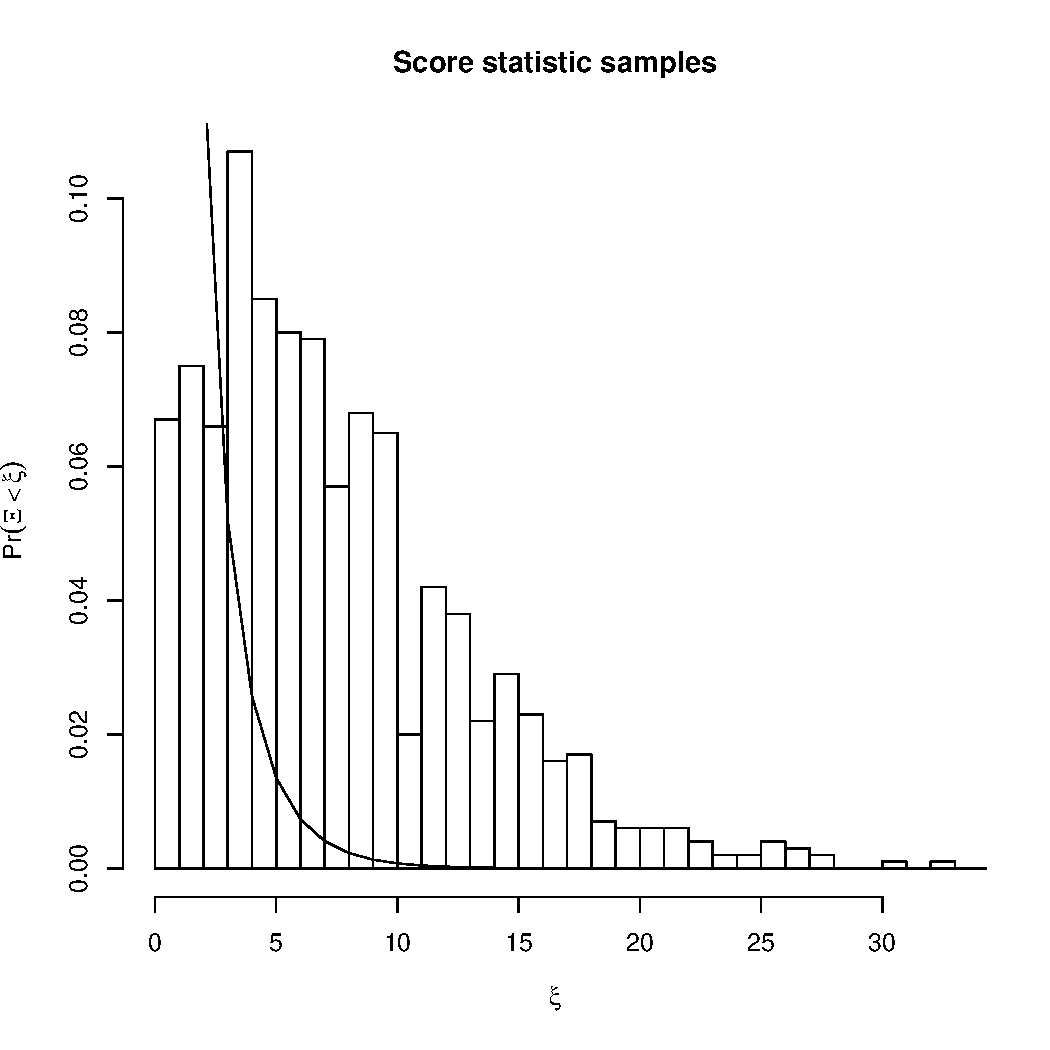
\includegraphics[scale=0.6]{hist.pdf}
\end{center}
\end{figure}


\section{An algorithm for estimating $\phi$ and $\lambda$ with no covariates}

In this section we detail an algorithm for estimating the two parameters of a ZIP model that is readily programmable within a spreadsheet with basic arithmetic calculations. Although the algorithm contains a while loop that is potentially infinite, in our experience the number of iterations is typically no more than 5-10. Moreover, the calculations required in each iteration are readily programmed so that the researcher may apply the technique to various data via copy and paste to mimic the iterations of the while loop. The algorithm follows: 

\begin{algorithm}
\caption{Calculate $\hat{\phi}$ and $\hat{\lambda}$}
\label{EM_algo}
\begin{algorithmic}[1]
\For{$i \gets 1, n$}\\
	\State $w_i \gets U_i$
\EndFor
\end{algorithmic}
\end{algorithm}

A spreadsheet to accompany the manuscript is available to illustrate the necessary calculations as well as provide a working template for the nematologist. The spreadsheet is titled \texttt{phi\_lambda\_calc.xlsx} and is available in the supplementary material on the journal website. 

\section{Discussion}
In this brief research note we discussed the zero-inflated distributions and several statistical and scientific implications of nematodes using the standard statistical techniques when modeling nematode abundance with count data. We argue that all nematologists should be familiar with zero-inflated models and use these methods in place of the standard classical statistics to estimate rates of nematodes in soil volume data. Moreover we stressed the computational aspects of these methods as well as the statistical nuances of the methods. Finally we provided an algorithm to estimate the rate of nematodes under a zero-inflated model and the zero-inflation probability component as well as provided a spreadsheet with calculations ready programmed for the researcher to modify as needed for their nematode abundance data. 


\end{document}
